%\documentclass{report}
%\begin{document}

\chapter{Tmix: Internet Traffic Generation}
\label{chap:tmix}

In order to perform realistic network simulations, one needs a traffic generator that is capable of generating realistic synthetic traffic that ``looks like'' traffic found on an actual network. Tmix takes as input a packet header trace taken from a network link of interest. The trace is ``reverse compiled'' into a source-level characterization, called a \emph{connection vector}, of each TCP connection present in the trace.  This set of connection vectors is what drives the Tmix traffic generation in ns-2.  

Connection vectors are represented through a pattern of application data units (ADUs) which are based on the \emph{a-b-t} model \cite{weigle-ccr06}.  Modeling TCP connections as a pattern of ADU transmissions provides a unified view of connections that does not depend on the specific applications driving each TCP connection.  The first step in the modeling process is to acquire a trace of TCP/IP headers and process the trace to produce a set of connection vectors; one vector for each TCP connection in the trace.

The Tmix module in ns-2 takes a set of connection vectors and emulates the socket-level behavior of the source application that created the corresponding connection in the trace. This emulation faithfully reproduces the essential pattern of socket reads and writes that the original application performed without knowledge of what the original application actually was. When combined with Tmix\_DelayBox (Section \ref{sec:tmix-db}), the resulting traffic generated in the simulation is statistically representative of the traffic measured on the real link. All a user needs to replay traffic from a certain link is the file of \emph{a-b-t} style connection vectors obtained from a trace of that link and this Tmix generator. This approach to synthetic traffic generation allows one to automatically reproduce in ns-2 the full range of TCP connections found on an arbitrary link.

The remainder of this chapter describes the implementation and use of Tmix in ns-2.  For more details on the \emph{a-b-t} model and validation of the Tmix generator, see \cite{weigle-ccr06}.

\textbf{Citation Request:}  If you use Tmix traffic generation in your work, please cite \cite{weigle-ccr06} (M.C. Weigle, P. Adurthi, F. Hernandez-Campos, K. Jeffay, and F.D. Smith, ``Tmix: A Tool for Generating Realistic Application Workloads in ns-2'', \emph{ACM SIGCOMM Computer Communication Review}, July 2006, Vol 36, No 3, pp. 67-76.).

\textbf{Note:} For more information on Tmix and to obtain Tmix tools and connection vectors, see http://netlab.cs.unc.edu/Tmix.

\section{Network Setup}

The implementation of Tmix in ns-2 is based on PackMime-HTTP (Chapter
\ref{chap:packmime}), so it has a similar structure.  A typical
Tmix instance consists of four ns nodes: two initiator nodes and two
acceptor nodes (Figure \ref{fig:tmix}).  
\begin{figure}
\centering
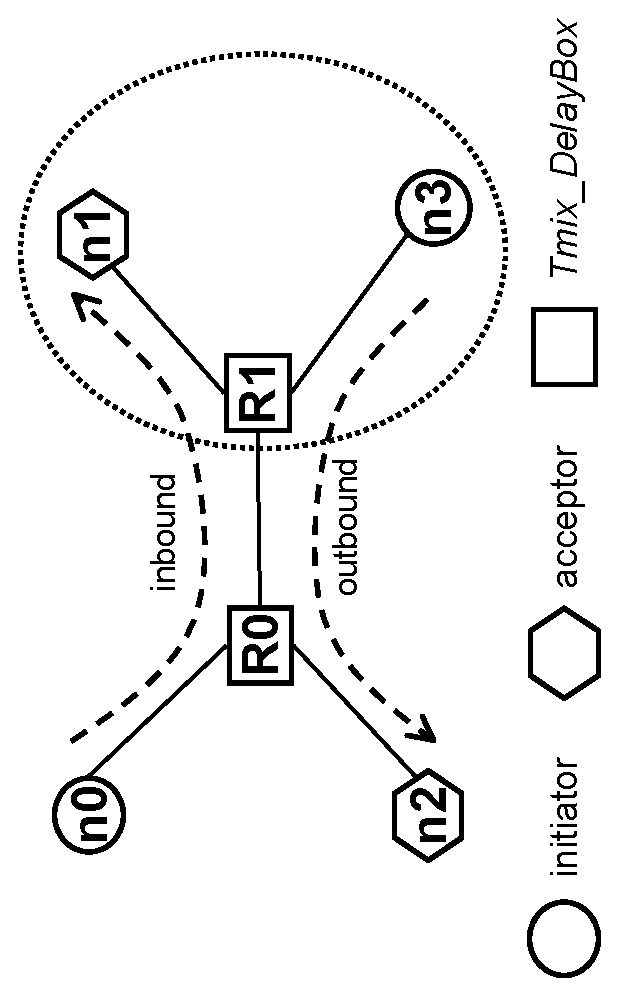
\includegraphics[scale=0.5, angle=270, clip]{tmix-fig.eps}
\label{fig:tmix}
\caption{Tmix Architecture. Each Tmix object controls
an initiator cloud and an acceptor cloud.  Each cloud can represent
multiple initiator or acceptor Applications.  For realistic two-way
traffic, two sets of acceptors and initiators are required.}
\end{figure}  
It is important to note that these nodes \emph{do not} correspond to a
single initiator or acceptor. A single Tmix initiator node generates
TCP connections coming from a ``cloud'' of connection initiators.
Likewise, a single Tmix acceptor node accepts and serves TCP
connections destined for a ``cloud'' of connection acceptors. 
%  A
% single initiator is represented by a single Tmix Application, and a
% single acceptor is represented by another instance of a single Tmix
% Application. There are many Tmix Applications assigned to a single
% initiator ns node, and many Tmix Applications assigned to a single
% acceptor ns node.

In order to simulate different RTTs, bottleneck links, and/or loss
rates for each connection, Tmix should be used in conjunction with
Tmix\_DelayBox (see Section \ref{sec:tmix-db}), derived from
DelayBox (Chapter \ref{chap:delaybox}).  

We use the terms \emph{inbound} and \emph{outbound} to represent the
directions of data flow.  As in Figure \ref{fig:tmix}, traffic
initiated outside of the circle (which could be thought of as a
campus) is designated as \emph{inbound}, and traffic initiated inside
the circle is designated as \emph{outbound}.

\section{Connection Vectors}

A connection vector is a representation of an observed TCP connection.
Each connection vector has several fields which specify the type of
connection (sequential or concurrent), connection start time, loss
rate, window size, etc.  Each connection vector also contains an
arbitrary number of application data units (ADUs).  Each ADU represents
data to be sent over the network by either the initiator or the
acceptor of the TCP connection.  ADUs also specify when data should be
sent relative to either the reception of an ADU or the completed
sending of a previous ADU.  A file containing an arbitrary number of
connection vectors must be supplied to Tmix in order for any traffic
to be generated.  

Connection vectors are either \emph{sequential} or \emph{concurrent}.
Sequential connection vectors are the most common and represent a
request-reply type connection, where a new ADU is sent only after the
previous ADU has been received.  Concurrent connection vectors allow
for deviation from the sequential pattern.  For a concurrent
connection, new ADUs are sent a certain amount of time after the
previous ADU was sent and do not depend upon when ADUs were
received. Examples of this type of application protocol include
HTTP/1.1 (pipelining) and the BitTorrent file-sharing protocol.

Tmix in ns-2 can handle two different connection vector formats, which
we term as \emph{original} and \emph{alternate}.  We have provided a Perl
script ({\tt ns/tmix/cvec-orig2alt.pl}) to convert from the original format to
the alternate format.  The Tmix module in ns-2 can automatically
detect the format of the given connection vector file.

%\emph{\textbf{Add section on how connection vectors can be obtained (1) using tools     %(obtained how?) to process a tcpdump trace and output connection vectors, or (2)     %writing a program to generate connection vectors by random sampling from     %distributions for connection start times, connection type, number of epochs,     %initiator/acceptor ADU sizes and delay times, etc.  }}

\subsection{Original Connection Vector Format}

Examples of the original format of connection vectors as described in
\cite{weigle-ccr06} are shown in Figure \ref{orig-cvec}.
\begin{figure}
\makebox[\columnwidth]{\hrulefill}
\small
\begin{verbatim}
SEQ 6851 1 21217 555382       # starts at 6.851 ms and contains 1 exchange (epoch)
w 64800 6432                  # win sz (bytes): init acc
r 1176194                     # min RTT (microseconds)
l 0.000000 0.000000           # loss: init->acc acc->init
> 245                         # init sends 245 bytes
t 51257                       # acc waits 51 ms after recv
< 510                         # acc sends 510 bytes
t 6304943                     # init waits 6.3 sec after send and then sends FIN

CONC 1429381 2 2 26876 793318 # starts at 1.4 s, init sends 2 ADUs and acc sends 2 ADUs
w 65535 5840                  # win sz (bytes)
r 36556                       # min RTT (microseconds)
l 0.000000 0.000000           # loss rate
c> 222                        # init sends 222 bytes
t> 62436302                   # init waits 62 sec
c< 726                        # acc sends 726 bytes
t< 62400173                   # acc waits 62 sec
c> 16                         # init sends 16 bytes
t> 725                        # init waits 725 us and then sends FIN
c< 84                         # acc sends 84 bytes
t< 130                        # acc waits 130 us and then sends FIN
\end{verbatim}
\makebox[\columnwidth]{\hrulefill}
\caption{\label{orig-cvec}Original Connection Vector Format Example.
In the comments, we abbreviate the initiator as \texttt{init} and the
acceptor as \texttt{acc}.}
\end{figure}
Sequential and concurrent connection vectors are differentiated by the
starting string in the first line: \texttt{SEQ} for a sequential
connection and \texttt{CONC} for a concurrent connection.  The second
field in the first line gives the starting time for the connection in
microseconds from time 0 (the start of the simulation).  For sequential connections, the third field indicates
the number of ADU exchanges, or \emph{epochs}, present in the
connection.  For concurrent connections, the third field indicates the
number of ADUs that the initiator sends, and the fourth field indicates
the number of ADUs that the acceptor sends. The final two fields in
the first line are identification numbers, of which only the final ID
is used in ns-2.

The second line in each, starting with \texttt{w}, gives the window
sizes of the initiator and acceptor, respectively, in bytes.  The
third line, starting with \texttt{r}, gives the minimum RTT in
microseconds between the initiator and acceptor.  The fourth line,
starting with \texttt{l}, provides the loss rates involved in each
direction of the connection. The remaining lines in the connection
vector show the ADU exchanges.

In a sequential connection vector, the ADUs are shown in increasing
order by the times at which they are sent.  The lines starting with
\texttt{$>$} show the sizes of the ADUs sent by the initiator
to the acceptor, and the lines starting with \texttt{$<$} show the
sizes of the ADUs sent by the acceptor to the initiator. Note
that there is a time dependency in case of sequential connection
vectors.  One side of the connection is dependent on the other side of
the connection sending it an ADU.

In case of sequential connections, the line containing
\texttt{t} can appear in any of the following four scenarios:
\begin{enumerate}
\item{After a line beginning with \texttt{$>$} and before a line
beginning with \texttt{$<$}}.
\item{After a line beginning with \texttt{$<$} and before a line
beginning with \texttt{$>$}}.
\item{At the end of the connection vector, after a line beginning with
\texttt{$>$}}.
\item{At the end of the connection vector, after a line beginning with
\texttt{$<$}}.
\end{enumerate}
Depending on its placement, the semantics associated with the
\texttt{t} value change. In case 1, \texttt{t} denotes the amount of
time the acceptor has to wait after receiving an ADU from initiator
before it can send its next ADU\@. In case 2, the \texttt{t} denotes
the amount of time the initiator has to wait after receiving an ADU
from acceptor before it can send its next ADU\@. In case 3, the
\texttt{t} denotes the time the initiator has to wait after sending
its last ADU and before closing the connection. In case 4, the
\texttt{t} denotes the time that the acceptor has to wait after
sending its last ADU and before closing the connection.

For a concurrent connection vector, lines starting with \texttt{c$>$}
indicate the bytes sent by the initiator, and lines starting with
\texttt{c$<$} indicate the bytes sent by the acceptor.  Lines starting
with \texttt{t$>$} indicate the time the initiator waits before
sending the next ADU (or sending the FIN, if the last ADU has been
sent).  Likewise with lines beginning with \texttt{t$<$} and the
acceptor.  Note that there is no time dependence between the initiator
and acceptor in case of a concurrent connection vector.  The waiting
times are between consecutive sends and are not dependent upon
receiving an ADU from the other side.

\subsection{Alternate Connection Vector Format}

To disambiguate the multiple possible interpretations of the
\texttt{t} value with sequential connections, we have modified the
connection vector format into an alternate format.  The basic idea is
that in the case of sequential connection vectors, there really exist
two times associated with the initiator or acceptor while sending an
ADU to the other side:
\begin{enumerate}
\item{The amount of time the initiator/acceptor has to wait before
sending the next ADU after sending its previous ADU
(\emph{send\_wait\_time}).} 
\item{The amount of time the initiator/acceptor has to wait before
sending the next ADU after receiving an ADU from the other side
(\emph{recv\_wait\_time}).}
\end{enumerate}
Note that only one of the above two values is used by an
initiator/acceptor while sending its ADU to the other side,
\emph{i.e.}, the initiator/acceptor schedules sending its next ADU
with respect to the event of receiving a ADU from the other side or
with respect to the event of sending a previous ADU.  The
initiator/acceptor does not use both of these values at the same time,
so in the new format one of these values is always set to 0. Also note
that at the beginning of the connection, the side sending the first
ADU will have both \emph{send\_wait\_time} and \emph{recv\_wait\_time}
set to 0. In case of the \texttt{t} values appearing at the end of a
connection vector in the original format, we introduce a dummy ADU
with size 0 to represent the FIN that will be sent by the
initiator/acceptor that sends the last ADU.

This same alternate representation can be used for concurrent
connection vectors also.  But because there is no time dependence
between the sides of the connection, each side schedules sending its
next ADU with respect to time at which it sent its last
ADU. Therefore, in case of concurrent connection vectors,
\emph{recv\_wait\_time} is not applicable and is always set to
0. Also, in case of concurrent connection vectors, both the sides
start sending their messages at the same time.

We keep the header lines of the connection vectors (those containing
the start time, window size, RTT, and loss rates) in the same format
as the original, except that we replace \texttt{SEQ} with \texttt{S}
and \texttt{CONC} with \texttt{C}\@.  Lines beginning with \texttt{I}
denote actions for the initiator, and lines beginning with \texttt{A}
show actions for the acceptor.  The remaining format of these lines is
\texttt{send\_wait\_time recv\_wait\_time bytes}.  Figure
\ref{alt-cvec} shows the alternate connection vector format
corresponding to the sequential and concurrent connections shown in
Figure \ref{orig-cvec}.

\begin{figure}
\makebox[\columnwidth]{\hrulefill}
\small
\begin{verbatim}
S 6851 1 21217 555382       # starts at 6.851 ms and contains 1 exchange (epoch)
w 64800 6432                # win sz (bytes)
r 1176194                   # min RTT
l 0.000000 0.000000         # loss rate
I 0 0 245                   # init sends 245 bytes
A 0 51257 510               # acc waits 51.257 ms after recv then sends 510 bytes
A 6304943 0 0               # acc waits 6.3 sec after send then sends FIN

C 1429381 2 2 26876 793318  # starts at 1.4 s, init sends 2 ADUs and acc sends 2 ADUs
w 65535 5840                # win sz (bytes)
r 36556                     # min RTT
l 0.000000 0.000000         # loss rate
I 0 0 222                   # init sends 222 bytes
A 0 0 726                   # acc sends 726 bytes
I 62436302 0 16             # init waits 62 sec and then sends 16 bytes
A 62400173 0 84             # acc waits 62 sec and then sends 84 bytes
I 725 0 0                   # init waits 725 us and then sends FIN
A 130 0 0                   # acc waits 130 us and then sends FIN
\end{verbatim}
\makebox[\columnwidth]{\hrulefill}
\caption{\label{alt-cvec}Alternate Connection Vector Example.
In the comments, we abbreviate the initiator as \texttt{init} and the
acceptor as \texttt{acc}.}
\end{figure}

\section{Implementation Details}

Tmix is an ns object that drives the generation of TCP traffic. Each
Tmix object controls the operation of two applications: a Tmix
Application used to simulate a TCP connection acceptor and a Tmix
Application used to simulate a TCP connection initiator. Each of these
applications is connected to a TCP Agent (Full-TCP).  {\bf Note:} Tmix
currently only supports Full-TCP agents, but one-way TCP support is under development.

Each initiator or acceptor cloud is represented by a single ns node
that can produce and consume multiple TCP connections at a time
(Figure \ref{fig:tmix}). For each TCP connection, Tmix creates (or
allocates from the inactive pool, as described below) initiator and
acceptor applications and their associated TCP Agents. After setting up
and starting each connection, Tmix sets a timer to expire when
the next new connection should begin. The times at which connections begin
are governed by the connection vectors supplied by the user.  Connection
vectors may be specified by the user by setting a connection vector file for 
Tmix to read from.  New connections are started according to the connection 
arrival times found in the connection vector file, without regard to the 
completion of previous connections.

Tmix handles the re-use of applications and Agents that have
completed their data transfer. There are 5 pools used to maintain
applications and Agents -- one pool for inactive TCP Agents and one
pool each for active and inactive Tmix Application. The
pools for active applications ensure that all active applications are
destroyed when the simulation is finished. Active TCP Agents do not
need to be placed in a pool because each active application contains a
pointer to its associated TCP Agent. New objects are only created when
there are no Agents or applications available in the inactive pools. 

\subsection{Tmix Application}

There is only one Tmix Application class.  This class is responsible for
handling both the initiator and acceptor roles, although different instances
of this class are used for each role, \emph{i.e.}, one object does
not handle both the initiator and acceptor roles at the same time.

The behavior of the Tmix Application class is in large part controlled by
the connection vectors found in the connection vector file set by
the user.  Each connection vector specifies the data to be sent by the initiator
and acceptor applications and under what conditions that data should be sent.

% \subsection{Tmix Application - Initiator}

% A Tmix Application in the role of the initiator generates TCP traffic by
% taking the following actions:

% \begin{itemize}
% \item{connect to the acceptor application associated with this application}
% \item{if the connection is sequential, new data is scheduled to be sent every
% time some new data is received}
% \item{if the connection is concurrent, new data is scheduled to be sent after
% the previous send by the same application}
% \item{once both applications have finished sending their data, close the
% connection}
% \end{itemize}

% Details on how data is sent for sequential and concurrent connections can be 
% found immediately following the next section.

% \subsection{Tmix Application - Acceptor}

% A Tmix Application in the role of the acceptor generates TCP traffic by
% taking the following actions:

% \begin{itemize}
% \item{listen for a connection from the associated initiator application}
% \item{if the connection is sequential, new data is scheduled to be sent every
% time some new data is received}
% \item{if the connection is concurrent, new data is scheduled to be sent after
% the previous send}
% \item{once both applications have finished sending their data, close the
% connection}
% \end{itemize}

% Details on how data is sent for sequential and concurrent connections are 
% provided in the two following sections.

\subsection{Sequential Connections}

The first ADU that has a 0 value for both \emph{recv\_wait\_time} and
\emph{send\_wait\_time} is sent as soon as the connection is initiated.
All following sends only occur after the initiator or acceptor
application has received the expected amount of data from its peer
(\emph{i.e.}, the initiator or acceptor application to which it is connected)
and after some delay specified by the next ADU to be sent. The
expected amount of data to be received from the peer is determined by
looking at the size of the current ADU that should be being sent by
the peer application.

\subsection{Concurrent Connections}

Both sides begin sending their data after the delay specified by their
ADUs. Later sends are scheduled to occur after the current send
has finished and after some delay specified by the next ADU to be
sent.

\subsection{Acceptor-Sending-First Connections}
There are some connections where the acceptor sends the first ADU\@.  In reality, the initiator always sets up the TCP connection, but in ns-2 the connection is not setup until the first data bytes are sent.  In these cases, the acceptor will send the SYN to setup the connection and then will send its ADU\@.

\section{Tmix\_DelayBox}
\label{sec:tmix-db}

Tmix uses ns-2 to model the TCP-level interaction between two nodes on
the simulated link. To simulate network-level effects of TCP transfer
through the clouds, use Tmix\_DelayBox. Tmix\_DelayBox is derived from
DelayBox (Chapter \ref{chap:delaybox}).  Tmix\_DelayBox simply adds
the ability to specify delays and losses for each connection using a
connection vector file instead of making setting up rules for each
source-destination pair.  After a connection vector file is specified,
Tmix\_DelayBox parses each connection vector to obtain the loss rate and
delay, which are written into the DelayBox flow table.  Note that the current version of Tmix\_DelayBox does not allow bandwidth limitations as does DelayBox, but that future versions may support this.

\section{Example}
The following is an example of using Tmix and Tmix\_DelayBox.  Another example can be found at {\tt tcl/ex/tmix/test-tmix.tcl}.  The
validation script {\tt test-suite-tmix.tcl} is in {\tt tcl/test/} and
can be run with the command {\tt test-all-tmix} from that directory.

\begin{verbatim}
	# Simulation script to simulate the tmix-ns component

	#::::::::::: Useful Variables ::::::::::::::::::::::
	set end 3600;                       # length of traced simulation (s)
	set INBOUND "inbound.cvec"
	set OUTBOUND "outbound.cvec"

	#::::::::::: Setup Simulator ::::::::::::::::::::::
	remove-all-packet-headers;             # removes all packet headers
	add-packet-header IP TCP;              # adds TCP/IP headers
	set ns [new Simulator];                # instantiate the Simulator
	$ns use-scheduler Heap

	#::::::::::: Setup Topology ::::::::::::::::::::::
	# create nodes
	set n(0) [$ns node]
	set n(1) [$ns node]
	set n(2) [$ns node]
	set n(3) [$ns node]

	# create Tmix_DelayBox nodes
	set tmixNet(0) [$ns Tmix_DelayBox]
	$tmixNet(0) set-cvfile "$INBOUND" [$n(0) id] [$n(1) id]
	$tmixNet(0) set-lossless

	set tmixNet(1) [$ns Tmix_DelayBox]
	$tmixNet(1) set-cvfile "$OUTBOUND" [$n(3) id] [$n(2) id]
	$tmixNet(1) set-lossless

	# create links
	$ns duplex-link $n(0) $tmixNet(0) 1000Mb 0.1ms DropTail
	$ns duplex-link $n(2) $tmixNet(0) 1000Mb 0.1ms DropTail
	$ns duplex-link $tmixNet(0) $tmixNet(1) 1000Mb 0.1ms DropTail
	$ns duplex-link $tmixNet(1) $n(1) 1000Mb 0.1ms DropTail
	$ns duplex-link $tmixNet(1) $n(3) 1000Mb 0.1ms DropTail

	# set queue buffer sizes (in packets)  (default is 20 packets)
	$ns queue-limit $n(0) $tmixNet(0) 500
	$ns queue-limit $tmixNet(0) $n(0) 500
	$ns queue-limit $n(2) $tmixNet(0) 500
	$ns queue-limit $tmixNet(0) $n(2) 500
	$ns queue-limit $tmixNet(0) $tmixNet(1) 500
	$ns queue-limit $tmixNet(1) $tmixNet(0) 500
	$ns queue-limit $tmixNet(1) $n(1) 500
	$ns queue-limit $n(1) $tmixNet(1) 500
	$ns queue-limit $tmixNet(1) $n(3) 500
	$ns queue-limit $n(3) $tmixNet(1) 500
	
	#::::::::::: Setup TCP ::::::::::::::::::::::
	Agent/TCP/FullTcp set segsize_ 1460;           # set MSS to 1460 bytes
	Agent/TCP/FullTcp set nodelay_ true;           # disabling nagle
	Agent/TCP/FullTcp set segsperack_ 2;           # delayed ACKs
	Agent/TCP/FullTcp set interval_ 0.1;           # 100 ms

	#::::::::::: Setup Tmix ::::::::::::::::::::::
	set tmix(0) [new Tmix]
	$tmix(0) set-init $n(0);                 # name $n(0) as initiator
	$tmix(0) set-acc $n(1);                  # name $n(1) as acceptor
	$tmix(0) set-ID 7
	$tmix(0) set-cvfile "$INBOUND"

	set tmix(1) [new Tmix]
	$tmix(1) set-init $n(3);                 # name $n(3) as initiator
	$tmix(1) set-acc $n(2);                  # name $n(2) as acceptor
	$tmix(1) set-ID 8
	$tmix(1) set-cvfile "$OUTBOUND"

	#::::::::::: Setup Schedule ::::::::::::::::::::::
	$ns at 0.0 "$tmix(0) start"
	$ns at 0.0 "$tmix(1) start"
	$ns at $end "$tmix(0) stop"
	$ns at $end "$tmix(1) stop"
	$ns at [expr $end + 1] "$ns halt"

	$ns run
\end{verbatim}

\section{Commands at a Glance}
The following commands on the Tmix class can be accessed from OTcl:

{\tt [new Tmix]}\\
Creates a new Tmix instance.

{\tt \$tmix start}\\
Start Tmix

{\tt \$tmix stop}\\
Stop Tmix

{\tt \$tmix set-init <node>}\\
Set the initiator node on which the connection initiator applications will be run

{\tt \$tmix set-acc <node>}\\
Set the acceptor node on which the connection acceptor applications will be run

{\tt \$tmix set-outfile <filename>}\\
Outputs the results of the {\tt active-connections} and {\tt
  total-connections} commands to the specified file instead of standard error

{\tt \$tmix set-cvfile <filename>}\\
Set the connection vector file from which to start and run connections

{\tt \$tmix set-ID <int>}\\
Set the NS id for this object

{\tt \$tmix set-run <int>}\\
Set the run number so that the RNGs used for the random variables will
use the same substream (see Chapter \ref{chap:math} on RNG for more details).

{\tt \$tmix set-debug <int>}\\
Set the debugging level:
% \begin{itemize}
% 	\item{2: Output: TCP Agent creation, TCP Agent assignment (from pool),
% 	Application creation, \\
% 	Application assignment (from pool), number of active and inactive
% 	Applications, Application completion time, connection establishment time}
% 	\item{3: Level 1 + \\
% 	Output: The move of TCP agents and Applications to the respective
% 	inactive pools \\
% 	and pool sizes}
% 	\item{4: Level 2 + \\
% 	Output: The reading of a connection vector by Tmix on a certain node
% 	and associated information (node name, connection vector id, connection
% 	vector start time, current time, number of connections currently running
% 	on the node)}
% \end{itemize}

{\tt \$tmix set-warmup <int>}\\
Sets at what time output should start.  Only used with {\tt set outfile}.

{\tt \$tmix set-TCP <protocol>}\\
Sets the TCP type (Reno, Newreno, or Sack) for all connections in the
client and server clouds - Reno is the default

{\tt \$tmix set-pkt-size <int>}\\
Size of packets to construct and send (TCP MSS)

{\tt \$tmix set-step-size}\\
Number of connection vector to read at a time from the supplied connection vector file

{\tt \$tmix active-connections}\\
Output the number of currently active connections to standard error or the
outfile if it has been set.

{\tt \$tmix total-connections}\\
Output the total number of completed connections to standard error or
the outfile if it has been set.


{\bf Tmix\_DelayBox Commands}

The following commands on the Tmix\_DelayBox class can be accessed
from OTcl (note that Tmix\_DelayBox inherits commands available for DelayBox):

{\tt [\$ns Tmix\_DelayBox]}\\
Creates a new Tmix\_DelayBox node.

{\tt \$tmix\_db set-cvfile <filename>}\\
Set the connection vector file from which to read the delays and loss rates for
each flow

{\tt \$tmix\_db set-lossless}\\
Do not induce any losses 

{\tt \$tmix\_db set-debug <int>}\\
Set the debugging level
% \begin{itemize}
% \item{1: Output when packets are dropped at DelayBox}
% \item{2: Level 1 + \\
% Contents of the queue at each queue operation
% }
% \end{itemize}

%\end{document}
